\documentclass[12pt,a4paper]{article}

% Packages
\usepackage[utf8]{inputenc}    % Encoding
\usepackage[T1]{fontenc}       % Font encoding
\usepackage{lipsum}            % Dummy text (optional)
\usepackage{amsmath, amssymb}  % Math symbols
\usepackage{graphicx}          % For images
\usepackage{hyperref}          % Clickable links
\usepackage{enumitem}
\usepackage[a4paper, top=2cm, bottom=2cm, left=2cm, right=2cm]{geometry} % the margins


% Title info
\title{RDFIA Reports: tp 1, 2 and 3}
\author{Titouan Guerin \& Yacine Chettab}
\begin{document}
\date{\today}
\maketitle

\section{Theoretical foundation}

\subsection{Supervised Dataset}

\paragraph{Questions} 

\begin{enumerate}
    \item \textbf{$\star$ What are the train, val and test sets used for?} \newline
    The train set is used to train the model, 
    the validation set is used to tune the hyperparameters during the training of the model, 
    and the test set is used to evaluate the model's performance 
    (data that is not in the train set, so not seen by the model previously).

    \item \textbf{What is the influence of the number of examples $N$?} \newline
    The number of examples $N$ influences the model's ability to generalize, which means that by seeing
    enough examples, the model can learn to make predictions on unseen data. On the other hand, if 
    $N$ is too little, then the model will do more of a memorization of the training data, so it does not
    actually learn to generalize the problem. However, having too many samples $N$ can be a problem in terms 
    of training time and computational resources.
\end{enumerate}

\subsection{Network Architecture (forward)}

\paragraph{Questions}

\begin{enumerate}[resume]
    \item \textbf{Why is it important to add activation functions between linear transformations?} \newline
    Having no activation functions between the linear layers would make the whole network linear 
    (which is not what we are looking for). Chaining linear transformations is the same as having one linear
    layer but with just more weights. So the activation functions allow the network to learn non-linear
    patterns in the data.

    \item \textbf{$\star$ What are the sizes $n_x$, $n_h$, $n_y$ in the figure 1? In practice, how are these sizes chosen?}
    \begin{itemize}
        \item $n_x$ is the size of the input layer, the number of features for one data point,
        \item $n_h$ is the size of the hidden layer, a hyperparameter that is determined before training,
        \item $n_y$ is the size of the output layer, the number of classes for classification problems.
    \end{itemize}

    \item \textbf{What do the vectors $\hat{y}$ and $y$ represent? What is the difference between these two quantities?} \newline
    The vector $\hat{y}$ represents the predicted output of the model, while $y$ represents the true labels.

    \item \textbf{Why use a SoftMax function as the output activation function?} \newline
    The SoftMax function maps the output of the neural network to a probability distribution.
    This means that all the values outputted by the model are mapped between 0 and 1, and the sum
    of all the values are equal to 1: $\sum_{i=1}^{n} \hat{y}_i = 1$.

    \item \textbf{Write the mathematical equations allowing to perform the forward pass of the neural network, i.e.
allowing to successively produce $\tilde{h}$, $h$, $\tilde{y}$ and $\hat{y}$ starting at $x$.} 
    \begin{itemize}
        \item $\tilde{h} = W_h x + b_h$
        \item $h = \text{ReLU}(\tilde{h})$
        \item $\tilde{y} = W_y h + b_y$
        \item $\hat{y} = \text{SoftMax}(\tilde{y})$
    \end{itemize}
\end{enumerate}

\subsection{loss function}

\paragraph{Questions}

\begin{enumerate}[resume]
    \item \textbf{During training, we try to minimize the loss function. For cross entropy and squared error, how must
the $\hat{y}_i$ vary to decrease the global loss function $\mathcal{L}$?} \newline
    For the MSE, the prediction $\hat{y}$ is compared directly to $y$, so to minimize the loss, 
    we want the difference between those two values to be as small as possible. In this case we work 
    with real numerical values. This loss works for both regression and classification problems. \newline
    On the other hand, for the cross-entropy, we are working exclusively with probabilities, so to minimize the loss,
    we want the predicted probability $\hat{y}_i$ of the true class to be as close to 1 as possible,
    (and the predicted probabilities of the other classes to be as close to 0 as possible). Here $y$ is just a 
    probability vector, with just zeros except for the true class which is 1.

    \item \textbf{How are these functions better suited to classification or regression tasks?} \newline
    MSE is naturally suited to regression, since its gradient is linear in the prediction error, 
    providing a good measure of how far the prediction is from the target. 
    However, in classification this linear behavior is less effective, because it does not 
    properly penalize cases where the model is very confident but wrong (not enough at least).  

    Cross-entropy, on the other hand, has a gradient that grows rapidly 
    when the predicted probability for the correct class is small. 
    Basically you want to penalize a confident but wrong prediction because it impacts the other predicted probabilities.
    Since the penalty (or cost) of CE is logarithmic, and hence more harsh on wrong predictions,
    the gradient of the loss is larger and allows the model to learn faster.

    \begin{figure}[h]
        \centering
        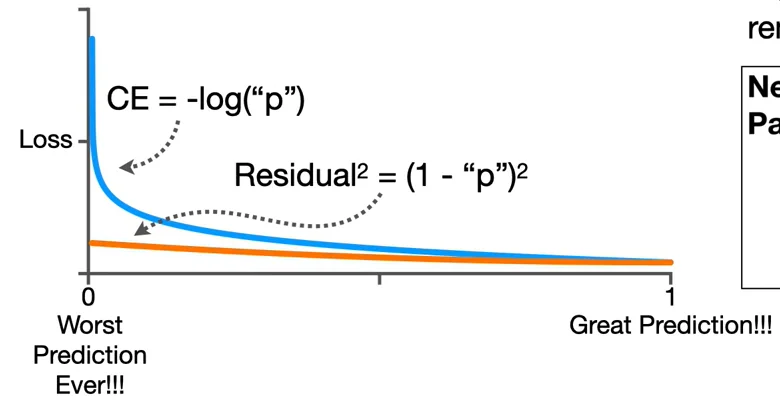
\includegraphics[width=0.4\textwidth]{CEillustration.png}
        \caption{\protect\href{https://www.reddit.com/r/learnmachinelearning/comments/yyfhm4/understanding_statquest_video_why_cross_entropy/}{Cross-Entropy vs MSE derivative comparison.}}
        \label{fig:ce_vs_mse}
    \end{figure}

\end{enumerate}

\subsection{Optimization algorithm}

    \paragraph{Questions}

    \begin{enumerate}[resume]
        \item \textbf{What seem to be the advantages and disadvantages of the various variants of gradient descent
                    between the classic, mini-batch stochastic and online stochastic versions? Which one seems the most
                    reasonable to use in the general case?} \newline
        TODO 
    \end{enumerate}

\end{document}